\documentclass[tikz]{standalone} 



\usepackage{tikz} 


\usetikzlibrary{arrows.meta}
\usetikzlibrary{patterns}
%\usetikzlibrary{backgrounds}
%\usetikzlibrary{shadows.blur}
\usepackage{xcolor}
\definecolor{myorange}{HTML}{FFA82E}  
\definecolor{myorange2}{HTML}{FFBB5C} 
\definecolor{myorange3}{HTML}{FFCE8A} 
\definecolor{background}{HTML}{FFE1B8}
\definecolor{gray}{HTML}{ADADAD}
\definecolor{gray2}{HTML}{969696}
\definecolor{darkgray}{HTML}{696969}
\definecolor{darkgray2}{HTML}{525252}
\definecolor{dark}{HTML}{3B3B3B}

\begin{document} 

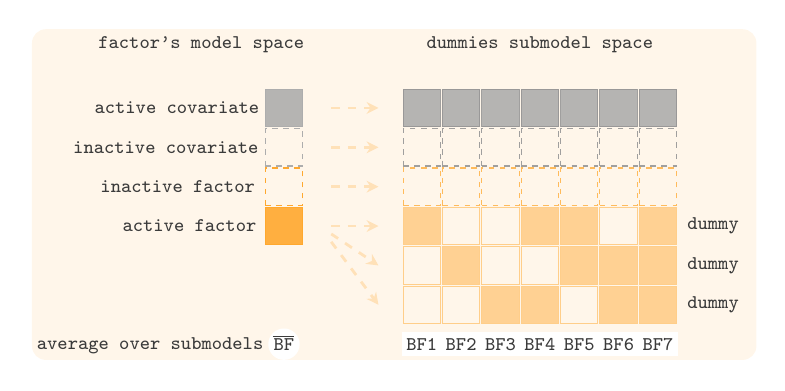
\begin{tikzpicture} 

%background color
\fill[background!30, rounded corners=5pt]
    (-1.2,-0.2) rectangle (8,4);

%node stiles
\tikzset{
    neuron2/.style={
        opacity=0.9,
        text opacity=0,
        draw opacity=0.9,
        rectangle=1pt,
        fill=darkgray,
        text=darkgray
    }
}

\tikzset{
    neuron2/.style={
        opacity=0.9,
        text opacity=0,
        draw opacity=0.9,
        rectangle=1pt,
        fill=gray,
        text=gray
    }
}

\tikzset{
    neuron/.style={
        opacity=0.9,
        text opacity=0,
        draw opacity=1,
        rectangle=1pt
    }
}

%main model space:
% row 0
\node[neuron2,draw=gray,fill=gray,text=gray,
    text width=0.24cm,text height=0.24cm,
    rectangle,text centered] at (2,3) {.};

% row 1
\node[neuron2,draw=gray,draw opacity=1,
    dash pattern=on 2pt off 2pt,
    fill=background!30,text=background!30,
    text width=0.24cm,text height=0.24cm,
    rectangle,text centered] at (2,2.5) {.};

% row 2
\node[neuron2,draw=myorange,draw opacity=1,
    dash pattern=on 2pt off 2pt,
    fill=background!30,text=background!30,
    text width=0.24cm,text height=0.24cm,
    rectangle,text centered] at (2,2) {.};

% row 3
\foreach \x in {2}{
    \node[neuron,draw=myorange,fill=myorange,text=myorange,
        text width=0.24cm,text height=0.24cm,
        rectangle,text centered] at (\x,1.5) {.};
}

%text
\node[text=dark, font=\scriptsize\bfseries\ttfamily] at (0.64,3) {active covariate};
\node[text=dark, font=\scriptsize\bfseries\ttfamily] at (0.5,2.5) {inactive covariate};
\node[text=dark, font=\scriptsize\bfseries\ttfamily] at (0.65,2) {inactive factor};
\node[text=dark, font=\scriptsize\bfseries\ttfamily] at (0.8,1.5) {active factor};
\node[text=dark, font=\scriptsize\bfseries\ttfamily] at (0.3,-0.02) {average over submodels};

\node[text=dark, font=\scriptsize\bfseries\ttfamily] at (7.45,1.5) {dummy};
\node[text=dark, font=\scriptsize\bfseries\ttfamily] at (7.45,1) {dummy};
\node[text=dark, font=\scriptsize\bfseries\ttfamily] at (7.45,0.5) {dummy};


\node[circle,
    fill=white,
    draw=none,
    text=dark, font=\scriptsize\bfseries\ttfamily,
    inner sep=1pt] at (2,0) {BF};
%overline first BF
%\node[text=myorange, font=\Large\ttfamily] at (10.75,2.1) {-};
\draw[dark, line width=0.4pt]
    (1.86,0.1) -- (2.13,0.1);

\fill[white] (3.5,-0.15) rectangle (7,0.15);

\node[text=dark, font=\scriptsize\bfseries\ttfamily] at (3.75,0) {BF1};
\node[text=dark, font=\scriptsize\bfseries\ttfamily] at (4.25,0) {BF2};
\node[text=dark, font=\scriptsize\bfseries\ttfamily] at (4.75,0) {BF3};
\node[text=dark, font=\scriptsize\bfseries\ttfamily] at (5.25,0) {BF4};
\node[text=dark, font=\scriptsize\bfseries\ttfamily] at (5.75,0) {BF5};
\node[text=dark, font=\scriptsize\bfseries\ttfamily] at (6.25,0) {BF6};
\node[text=dark, font=\scriptsize\bfseries\ttfamily] at (6.75,0) {BF7};

%submodel space

% header
% row 1
\foreach \x in {3.75,4.25,4.75,5.25,5.75,6.25,6.75}{
    \node[neuron2,draw=gray2,
        text width=0.24cm,text height=0.24cm,
        rectangle,text centered] at (\x,3) {.};
}

% row 1
\foreach \x in {3.75,4.25,4.75,5.25,5.75,6.25,6.75}{
    \node[neuron2,draw=gray2,
        dash pattern=on 2pt off 2pt,
        %pattern=north east lines,
        %pattern color=gray,
        fill=background!30,
        text width=0.24cm,text height=0.24cm,
        rectangle,text centered] at (\x,2.5) {.};
}

% row 2
\foreach \x in {3.75,4.25,4.75,5.25,5.75,6.25,6.75}{
    \node[neuron,draw=myorange2,
    dash pattern=on 2pt off 2pt,
        %pattern=north east lines,
        %pattern color=gray,
        fill=background!30,
        text width=0.24cm,text height=0.24cm,
        rectangle,text centered] at (\x,2) {.};
}

% row 3
\foreach \x in {3.75,4.25,4.75,5.25,5.75,6.25,6.75}{
    \node[neuron,draw=myorange3,
        text width=0.24cm,text height=0.24cm,
        rectangle,text centered] at (\x,1.5) {.};
}

\node[neuron,draw=myorange3,
    %dash pattern=on 2pt off 2pt,
        %pattern=north east lines,
        %pattern color=gray,
        fill=myorange3,
        text width=0.24cm,text height=0.24cm,
        rectangle,text centered] at (3.75,1.5) {.};

\node[neuron,draw=myorange3,
    %dash pattern=on 2pt off 2pt,
        %pattern=north east lines,
        %pattern color=gray,
        fill=myorange3,
        text width=0.24cm,text height=0.24cm,
        rectangle,text centered] at (5.25,1.5) {.};

\node[neuron,draw=myorange3,
    %dash pattern=on 2pt off 2pt,
        %pattern=north east lines,
        %pattern color=gray,
        fill=myorange3,
        text width=0.24cm,text height=0.24cm,
        rectangle,text centered] at (5.75,1.5) {.};

\node[neuron,draw=myorange3,
    %dash pattern=on 2pt off 2pt,
        %pattern=north east lines,
        %pattern color=gray,
        fill=myorange3,
        text width=0.24cm,text height=0.24cm,
        rectangle,text centered] at (6.75,1.5) {.};

% row 4
\foreach \x in {3.75,4.25,4.75,5.25,5.75,6.25,6.75}{
    \node[neuron,draw=myorange3,
        text width=0.24cm,text height=0.24cm,
        rectangle,text centered] at (\x,1) {.};
}

\node[neuron,draw=myorange3,
    %dash pattern=on 2pt off 2pt,
        %pattern=north east lines,
        %pattern color=gray,
        fill=myorange3,
        text width=0.24cm,text height=0.24cm,
        rectangle,text centered] at (4.25,1) {.};

\node[neuron,draw=myorange3,
    %dash pattern=on 2pt off 2pt,
        %pattern=north east lines,
        %pattern color=gray,
        fill=myorange3,
        text width=0.24cm,text height=0.24cm,
        rectangle,text centered] at (5.75,1) {.};

\node[neuron,draw=myorange3,
    %dash pattern=on 2pt off 2pt,
        %pattern=north east lines,
        %pattern color=gray,
        fill=myorange3,
        text width=0.24cm,text height=0.24cm,
        rectangle,text centered] at (6.25,1) {.};

\node[neuron,draw=myorange3,
    %dash pattern=on 2pt off 2pt,
        %pattern=north east lines,
        %pattern color=gray,
        fill=myorange3,
        text width=0.24cm,text height=0.24cm,
        rectangle,text centered] at (6.75,1) {.};

% row 5
\foreach \x in {3.75,4.25,4.75,5.25,5.75,6.25,6.75}{
    \node[neuron,draw=myorange3,
        text width=0.24cm,text height=0.24cm,
        rectangle,text centered] at (\x,0.5) {.};
}

\node[neuron,draw=myorange3,
    %dash pattern=on 2pt off 2pt,
        %pattern=north east lines,
        %pattern color=gray,
        fill=myorange3,
        text width=0.24cm,text height=0.24cm,
        rectangle,text centered] at (4.75,0.5) {.};

\node[neuron,draw=myorange3,
    %dash pattern=on 2pt off 2pt,
        %pattern=north east lines,
        %pattern color=gray,
        fill=myorange3,
        text width=0.24cm,text height=0.24cm,
        rectangle,text centered] at (5.25,0.5) {.};

\node[neuron,draw=myorange3,
    %dash pattern=on 2pt off 2pt,
        %pattern=north east lines,
        %pattern color=gray,
        fill=myorange3,
        text width=0.24cm,text height=0.24cm,
        rectangle,text centered] at (6.25,0.5) {.};

\node[neuron,draw=myorange3,
    %dash pattern=on 2pt off 2pt,
        %pattern=north east lines,
        %pattern color=gray,
        fill=myorange3,
        text width=0.24cm,text height=0.24cm,
        rectangle,text centered] at (6.75,0.5) {.};

%Write text

%upper text
\node[text=dark, font=\scriptsize\bfseries\ttfamily] at (0.95,3.8) {factor's model space};

\node[text=dark, font=\scriptsize\bfseries\ttfamily] at (5.25,3.8) {dummies submodel space};

%arrows:
\draw[ -{Stealth[length=1.5mm,width=1.5mm]}, draw=background, dashed , line width=1pt] (2.6,3) to
%[out=-20,in=80] 
(3.2,3);
\draw[ -{Stealth[length=1.5mm,width=1.5mm]}, draw=background, dashed , line width=1pt] (2.6,2.5) to
%[out=-20,in=80] 
(3.2,2.5);
\draw[ -{Stealth[length=1.5mm,width=1.5mm]}, draw=background, dashed , line width=1pt] (2.6,2) to
%[out=-20,in=80] 
(3.2,2);
\draw[ -{Stealth[length=1.5mm,width=1.5mm]}, draw=background, dashed , line width=1pt] (2.6,1.5) to
%[out=-20,in=80] 
(3.2,1.5);
\draw[ -{Stealth[length=1.5mm,width=1.5mm]}, draw=background, dashed , line width=1pt] (2.6,1.3) to
%[out=-20,in=80] 
(3.2,0.5);
\draw[ -{Stealth[length=1.5mm,width=1.5mm]}, draw=background, dashed , line width=1pt] (2.6,1.4) to
%[out=-20,in=80] 
(3.2,1);

\end{tikzpicture} 

\end{document}